\documentclass[a4paper,11pt]{report}
\usepackage[T1]{fontenc}
\usepackage[utf8]{inputenc}
\usepackage{lmodern}
\usepackage[francais]{babel}
\usepackage{graphicx}
\usepackage{array}

\title{Data wars}
\author{Guillaume LARROYENNE, Nathan PRETOT, Jeremy Renaud,Tom SALVI, Pierre VALENZA}

\begin{document}

\maketitle
\tableofcontents

\begin{abstract}
\end{abstract}

\chapter{Mise en Oeuvre}



\section{Rendu}
\subsection{Les composants du projet}
A ce jour, le projet comporte :

	\subsubsection{Un site web permettant :}
	
	 - De créer un compte utilisateur
		 
	 - De créer et modifier son deck de carte pour le jouer en jeu.
	 
	 - De télécharger le jeu.
	 
	 \begin{center}
	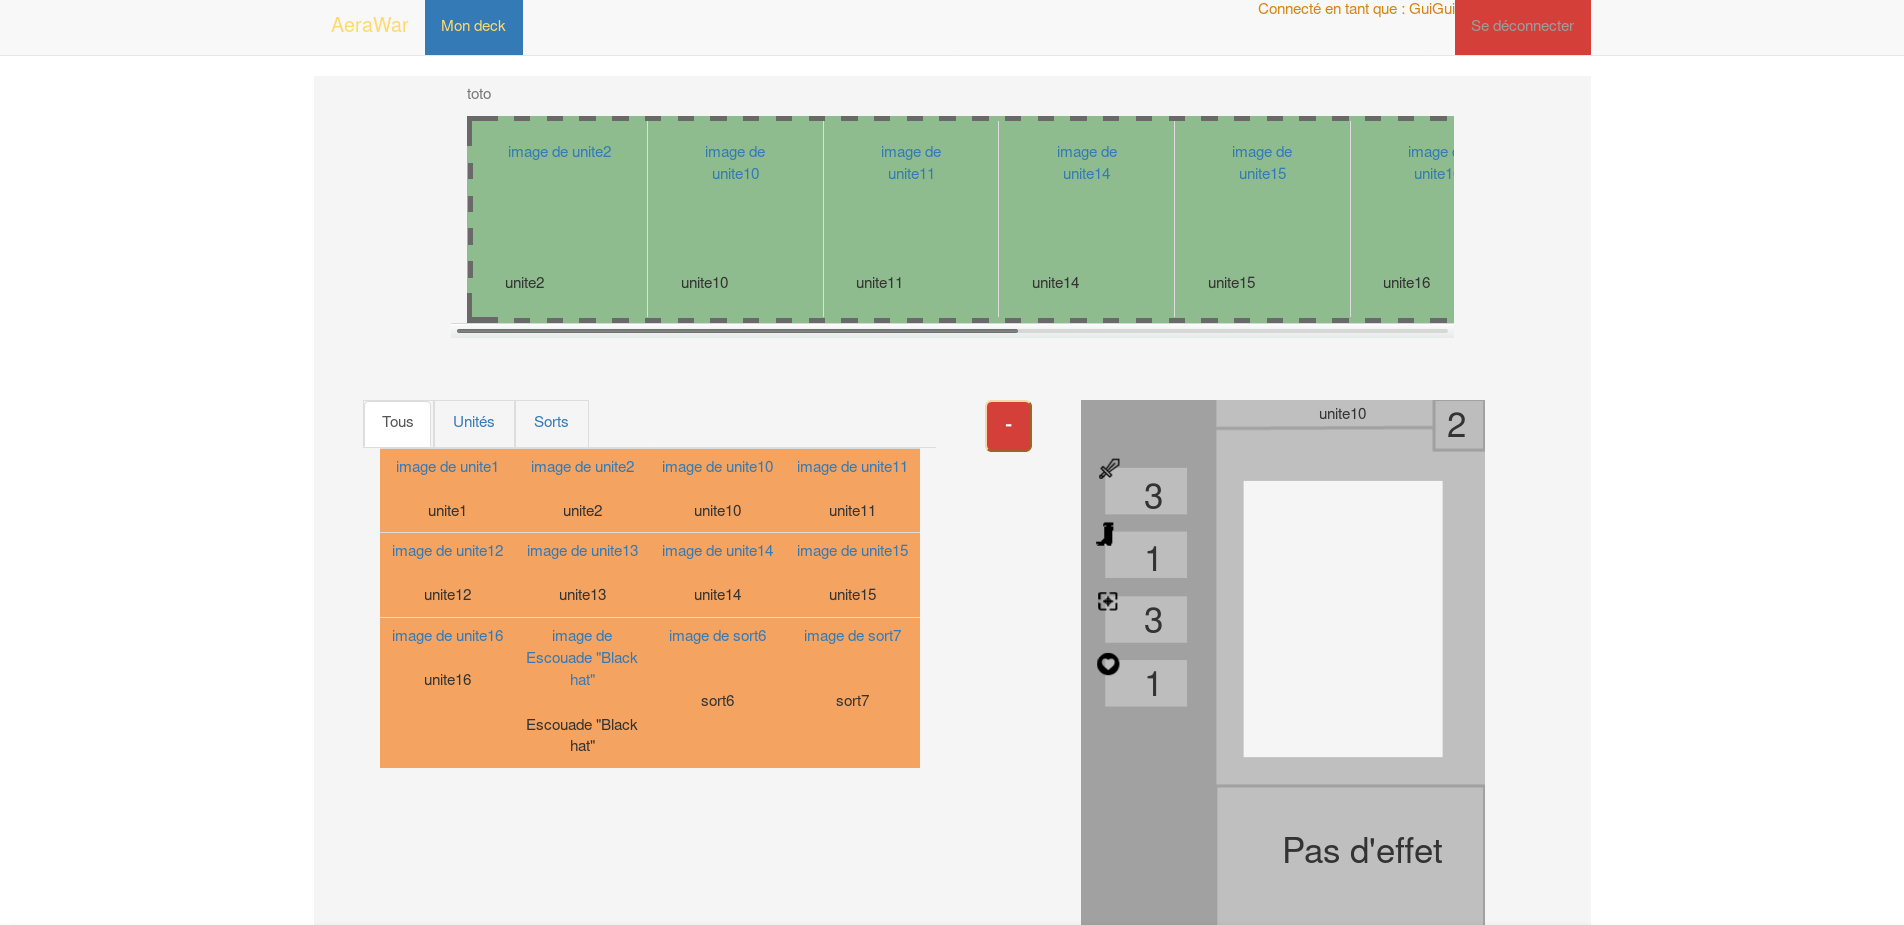
\includegraphics[scale=0.2]{Assets/site.png} 
	\end{center}

	
	\subsubsection{Un système réseau avec interface réutilisable\\ sur d'autres 			projets :}
	
	Il permet de créer un groupe, envoyer une invitation au membres connectés, ces derniers peuvent gérer les invitations reçus ( accepter ou non ) l'invitation est limitée dans le temps pour éviter d'attendre un joueur éternellement. Une fois le groupe créé l'hôte peut lancer la partie.   
	
	
	\begin{center}
	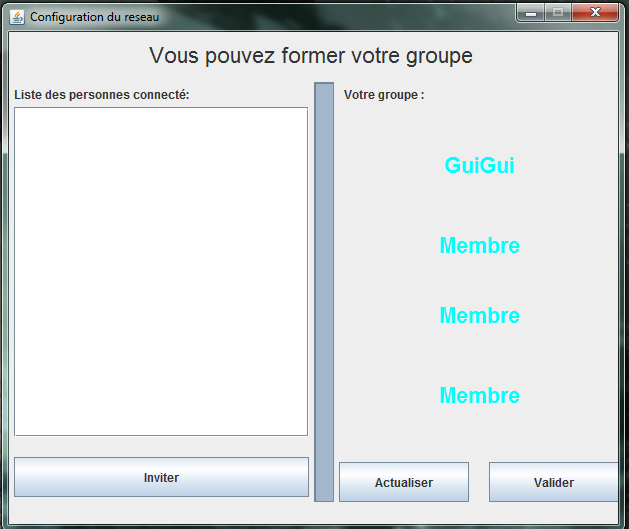
\includegraphics[scale=0.5]{Assets/connection3.png} 
	\end{center}
	
	\subsubsection{Un jeu jouable en Réseau de 2 à 4 joueurs.}
	
	Dans le jeu on peut récupérer le deck en fonction du joueur, jouer des cartes, déplacer des unités, attaquer des unités ennemies, capturer des bâtiments de ressources, voir les informations des entités sur la carte. La gestion des ressources est fonctionnelle.
	
	 On peut attaquer le QG ennemi pour gagner la partie.
	
 La partie de chaque joueur est synchronisée à chaque fin de tour d'un joueur.
	\begin{center}
	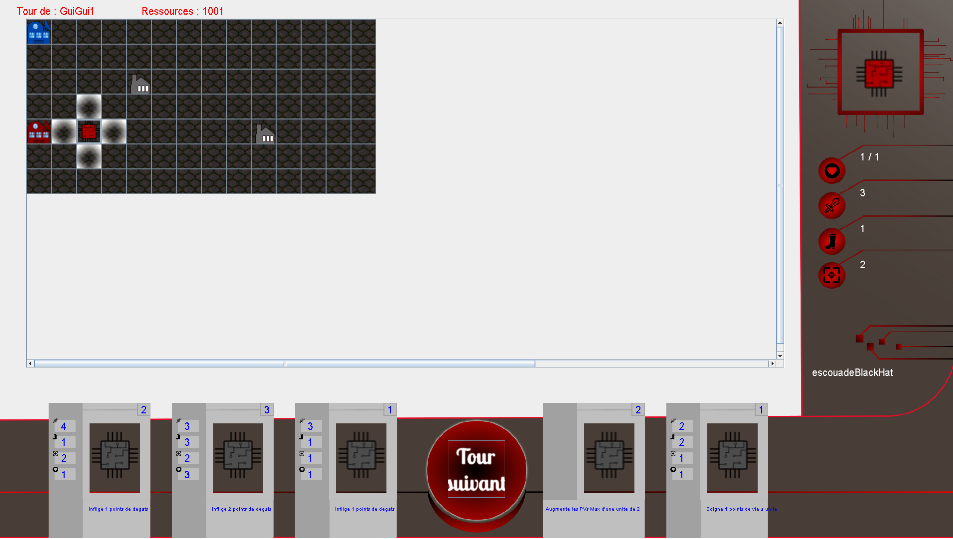
\includegraphics[scale=0.3]{Assets/UniteeSelectMove.png} 
	\end{center}
	


	

\end{document}
